\section{Related Work} \label{sec:related-work}

Traditionally, sound designers relied on manual labor to create audio, which involved recording and editing real-world sounds, mixing, and adding sound effects~\cite{sonnenschein_sound_2001}. Creating high-quality sounds is challenging, costly, and time-consuming, requiring specialized skills and resources. Hence, it engenders a notable impediment to the creation of soundscapes or any type of sound at scale~\cite{bernardes_seed_2016, strobl_sound_2006}, namely in light of its growing popularity and consumption within podcasts, movies, and video games.

Consumer data reported in 2021 showed compelling evidence regarding the listening habits of individuals within the United States of America. The findings indicate a substantial growth in podcast listenership over the past decade, with 41\% of Americans aged 12 or older having engaged with podcasts in the preceding month and 28\% within the last week. Moreover, at the beginning of the same year, a notable 68\% of Americans aged 12 and above had indulged in online audio consumption within the previous month, while 62\% had done so within the preceding week~\cite{research_infinite_2021}.

To overcome the aforementioned limitations, algorithmic audio generation has emerged as a promising solution that streamlines its creation altogether. Focusing on soundscapes, preceding 2018, prevailing models for their generation primarily revolved around statistical methods, featuring prominent employment of \ac{ML} techniques with feature engineering. For a comprehensive overview of techniques employed before the era of \ac{DL}, reference can be made to the review papers by Alias et al.\cite{alias_review_2016} and Kalonaris et al.\cite{kalonaris_computational_2018}. Noteworthy efforts at the feature engineering level are exemplified by Fernandez et al.~\cite{fernandez_ai_2013}, who represent sounds as high-level features, such as musical sheets, as an approach to generating musical sounds.

\Ac{DL} models for audio generation aim to produce high-quality audio signals by learning from existing audio data. Typically, these models consist of three main components: translation of the sound signal into a compressed representation, generation of a new representation from previous data, and translation back into an audio signal.

The first component of the model involves transforming the original sound signal into a Mel-spectrogram (or other) representation (see Section~\ref{sec:sound}), which is more compact and more accessible to process than the raw audio signal.

The second component involves generating new low-resolution representations from previous representations, such as spectrograms or feature vectors \cite{kong_hifi-gan_2020}. This is typically done using deep generative architectures. These models are trained on existing sound data to learn the target representation distribution and generate new, high-quality representations.

The final component of the model involves translating these representations back into an audio signal. These algorithms are called \textit{vocoders} (for more, see Section~\ref{sec:vocoders}). This component aims to produce high-quality audio signals that closely resemble the original sound data used to train the model.

The purpose of this section is to review the related work in this area. First, it examines the methods for generating traditional soundscapes, as described in Section~\ref{sec:trad-soundscape}. It then examines sound generation using machine learning. State-of-the-art models focus primarily on either using unsupervised sound generation techniques, as discussed in Section~\ref{sec:unsupervised-generation}, or generating sounds from internal representations, known as vocoders and discussed in Section~\ref{sec:vocoders}, or creating an end-to-end system, as discussed in Section~\ref{sec:end-to-end}.

\subsection{Traditional Soundscape Generation} \label{sec:trad-soundscape}

Feature engineering methods for soundscape generation typically adopt a threefold strategy to resynthesize (and extend) a short soundscape recording provided by the user:

\begin{enumerate}
    \item Segmentation,
    \item Feature extraction and modeling, and
    \item resynthesis of a given environmental sound.
\end{enumerate}

Statistical models adopting stochastic processes or pattern recognition methods were commonly applied to model and recreate a given soundscape recording with a degree of variation while maintaining its structure. Generated soundscapes relied on the similarity among audio segments to create smooth transitions~\cite{hoskinson_manipulation_2001}.

\subsubsection{Scaper}

Searching through the academic search engines, one finds that the most cited software for soundscape generation is \textit{Scaper} \cite{salamon_scaper_2017}.

Scaper is an open-source software library for soundscape generation designed to facilitate the creation of synthetic sound environments. It is a tool that allows users to simulate complex soundscapes, including urban, natural, and interior spaces, and investigate how various sound sources interact in these environments.

Scaper implements a modular soundscape generation framework based on basic sound-generating objects or ``sound sources''. These sound sources can represent simple sounds such as bird songs, human speech, or car horns, or more complex sounds like those produced by a crowd of people or a construction site. The user can specify the attributes of each sound source, such as its location, volume, and duration, and can adjust these parameters in real-time to create a dynamic soundscape.

One of the key features of Scaper is its ability to generate synthetic soundscapes that are diverse and statistically representative of real-world environments. To achieve this, the library implements various sound-generating algorithms that can be used to create sounds that are randomized yet realistic. For example, the library can generate sounds similar to real-world sources but with variations in volume, pitch, and timbre to avoid repetition and create a more diverse soundscape.

\subsubsection{SEED}

SEED is a system that addresses the formidable task of resynthesizing environmental sounds, such as city ambiances or nature scenes~\cite{bernardes_seed_2016}. SEED aims to provide a solution that not only extends the duration of environmental sounds but also provides precise control over the degree of variation in the output. This control over variation is critical in applications where maintaining the authenticity and coherence of the audio environment is essential.

SEED is built on a tri-partite architecture consisting of three main modules: segmentation, analysis, and generation. 

In the segmentation module, SEED performs the task of dividing the input audio into segments. This segmentation process is based on detecting spectral stability between frames. Spectral stability is a measure of how similar the frequency spectrum is between consecutive frames. When this stability falls below a certain threshold, it signals a change in the underlying sound source or event, prompting the placement of a segment boundary. This approach ensures that the resynthesized audio remains cohesive and retains its natural flow.

The Analysis module has two main processes. First, it extracts several audio features that capture both the sonic and temporal characteristics of the segments. These features are then clustered into a discrete ``dictionary'' of audio classes, effectively reducing the feature space to a finite set. At the same time, the module builds a transition table that records the sequences of these audio classes. This table is used to determine the probability that one class follows another.

In addition, the analysis module computes a concatenation cost matrix that quantifies how smoothly two segments can transition from one to the other. This matrix is computed by comparing the features at the segment boundaries. A lower cost indicates a smoother transition, while a higher cost indicates a more abrupt change.

In the Generation module, SEED generates new audio by searching for segment sequences that meet certain criteria. To achieve this, SEED references the transition table to determine viable next classes based on the current class in the audio sequence. It then assembles segments belonging to these classes and selects the one with the lowest concatenation cost. Notably, SEED applies a temporary cost penalty to recently selected segments to encourage diversity in the generated audio.

\subsubsection{Physics-Based Concatenative Sound Synthesis}

In the current development of virtual environments, the generation of audio content has been the subject of extensive research. One prominent approach in this area is \acf{CSS}, a method that creates novel auditory experiences by assembling segments of pre-existing sounds from a given database, often referred to as ``audio units''.

A recent scientific paper by Magalhães et al. presents an innovative \ac{CSS} framework based on physics-based principles for virtual reality~\cite{magalhaes_physics-based_2020}. This framework consists of two main components, namely the ``Capture Component'' and the ``Synthesis Component''.

The capture component of the framework is responsible for capturing essential data during interactions with virtual objects. This includes physics simulation data, haptic feedback data, position sensor data, and audio data. In particular, the physics data includes critical information such as collision points, velocities, impulses, and normals, among other parameters. The haptic and audio data are derived from real-world interactions with a variety of materials. This capture process culminates in the creation of a multimodal corpus of annotated audio units, which serves as the foundational resource for subsequent synthesis efforts.

The synthesis component of the framework uses the captured data to orchestrate the synthesis of auditory and haptic feedback by concatenating audio units extracted from the corpus. This unique mapping between physics data and audio units ensures congruence between user interactions and the resulting sensory feedback. For example, when a user applies a certain force and angle to interact with a virtual metal object, the synthesis component selects an audio unit recorded from a similar interaction with a real-world metal object.

At runtime, the framework relies on the target physics vectors to guide the selection of audio units, thus generating congruent auditory and haptic experiences. An overlap-add phase vocoder is used to concatenate the audio segments, while temporal repetition penalties are incorporated to ensure smooth transitions between these segments.
\subsection{Unsupervised Sound Generation} \label{sec:unsupervised-generation}

This Section focuses on models that address unsupervised or self-supervised training through learning sound features and their distributions without relying on explicit labels or annotations. In unsupervised sound generation, models learn from unlabeled audio data to capture underlying patterns and structures. This enables the generation of novel sound samples and the representation of latent features. This approach is particularly valuable when labeled datasets are scarce or expensive to acquire. Next, this discussion covers notable models in this area, selected based on their suitability for generating audio.

\subsubsection{WaveGAN} \label{sec:wavegan}

\Acp{GAN} have a notable impact on generating coherent images at the local and global levels, as discussed in Section~\ref{sec:gan}. A model based on \acp{GAN} called WaveGAN \cite{donahue_adversarial_2019} was proposed in 2019, to synthesize waveforms in an unsupervised manner. The model modifies the transposed convolution operation, used in \acp{DCGAN} for image generation, to capture waveform structure at different timescales.

WaveGAN modifies the transposed convolution operation in \acp{DCGAN}, expanding conventional \acp{GAN} to encompass image generation tasks and precisely capture the structure of audio signals of varying timescales. This model uses lengthier, one-dimensional filters of 25 units in place of two-dimensional filters with dimensions of $5 \times 5$. The model also upsamples each layer by a factor of 4, as is done in traditional \acp{DCGAN}. Despite these modifications, WaveGAN has the same number of parameters, numerical operations, and output dimensionality as \acp{DCGAN} have.

The experiments conducted on WaveGAN show that it can synthesize one-second slices of audio waveforms with global coherence, which is suitable for sound effect generation. The model also learns to produce intelligible words when trained on a small-vocabulary speech dataset without labels.

The success of WaveGAN in generating coherent audio signals demonstrates that \acp{GAN} can generate high-quality sounds. This work opens up new possibilities for unsupervised synthesis of raw-waveform audio, such as music and speech. It also suggests that \acp{GAN} can learn to capture the structure of signals across various timescales, which is crucial for generating realistic audio.

\subsubsection{Generative Transformer for Audio Synthesis}

In this work, Verma and Chafe~\cite{verma_generative_2021}, proposed in 2022, explore an alternative architecture using transformer networks (see Section~\ref{sec:transformers}), which have shown great success in sequential modeling tasks such as language translation.

The authors develop a generative transformer model for raw audio waveforms. The model is trained to autoregressively predict the next audio sample by attending over previous context samples. Specifically, the input waveform is split into overlapping frames and embedded into a latent space. A series of multi-headed causal self-attention layers then learn to focus on relevant parts of the input context to predict the subsequent sample distribution.

To retain information about the relative sample positions, positional encodings are added. Training deeper models is facilitated by layer normalization and residual connections. In a neural network, residual connections (also known as skip connections) enable the direct flow of information from one layer to subsequent layers. The use of residual connections helps to mitigate the vanishing gradient problem and allows for more effective gradient propagation during training. The inclusion of these connections enables the model to learn new representations at each layer and retain useful features from previous layers, resulting in improved performance and faster convergence. Self-attention provides the model with flexibility and frees it from the fixed topology of convolutions in other models such as WaveNet (Section~\ref{sec:wavenet}).

During training, previous samples are fed as input to the model to predict the next sample, optimized with cross-entropy loss (see Section~\ref{sec:cross-entropy}). The authors quantitatively evaluate next-step sample accuracy and find that the transformer architecture can outperform WaveNet baselines substantially.

\subsubsection{wav2vec 2.0}

The wav2vec 2.0 model comprises three essential components: a convolutional feature encoder, a Transformer network, and a quantization module. This model was originally introduced in the 2020 paper by Baevski et al. \cite{baevski_wav2vec_2020} and designed for speech generation tasks. For further details on the convolutional layer and the Transformer network, refer to Sections~\ref{sec:conv-layer} and \ref{sec:transformers}.

Quantization is the process of discretizing continuous values into a finite set of discrete symbols or codes, particularly in the context of generative models. This method is comparable to the technique used in the \ac{VQ-VAE} (refer to Section~\ref{sec:vq-vae}) In this technique, the input data is mapped to a limited number of discrete codebook entries.

For convolution, the feature encoder takes the raw audio waveform as input and generates a sequence of speech representations underlying it. This consists of several convolutional blocks, with each block including 1D temporal convolution and layer normalization. Wide kernels (\textit{e.g.,} 10ms) are used in the convolutions and progressively reduce the resolution of the input to extract hierarchical features.

The output of the feature encoder is fed into a transformer network to build contextualized representations. For encoding positional information specific to speech generation tasks, we use a convolutional layer instead of absolute positional embeddings. The self-attention mechanism enables each time step to consider all other time steps, thus capturing long-range dependencies in the sequence. Several Transformer layers extract higher levels of contextual abstraction.

A quantization module is applied to the output of the feature encoder. It discretizes the continuous latent representations into a finite inventory of speech units. Multiple codebooks are maintained, and concatenating selections from each codebook construct discrete units.

After pre-training on unlabeled speech, the model is fine-tuned on transcribed speech for speech recognition by adding a randomly initialized output layer. Various augmentations are used during fine-tuning to improve robustness.

The key innovations are the joint training of discrete speech units and contextualized representations in a completely self-supervised fashion. Experiments demonstrate strong performance even with just minutes of labeled data, highlighting the benefits of pre-training on large unlabeled corpora.

\subsubsection{SoundStream} \label{sec:soundstream}

SoundStream is a neural audio codec proposed in 2021 \cite{zeghidour_soundstream_2021} that can efficiently compress speech, music, and general audio. A codec is software or hardware that compresses and decompresses audio signals. The model architecture consists of a fully convolutional encoder/decoder network and a residual vector quantizer.

The fully convolutional encoder receives a time-domain waveform as input. It produces a sequence of embeddings at a lower sampling rate, which is then quantized by the \ac{RVQ}. The fully convolutional decoder then receives the quantized embeddings and reconstructs an approximation of the original waveform. Both the encoder and decoder use only causal convolutions, so the overall architectural latency of the model is determined solely by the temporal resampling ratio between the original time-domain waveform and the embeddings.

While there are similarities between SoundStream and a standard \ac{AE} (see Section \ref{sec:autoencoders}) in terms of the encoder-decoder architecture, SoundStream includes additional components such as the \ac{RVQ} and the use of structured dropout for variable bitrate compression.

A \acf{RVQ} is a vector quantization method. It is a variant of the traditional vector quantization method present, for instance, in \acp{VQ-VAE} (see Section \ref{sec:vq-vae}). In an \ac{RVQ}, the input data is first transformed into a lower-dimensional space using a neural network encoder. The resulting embeddings are then quantized using a codebook of fixed-size vectors, where each input embedding is assigned to the nearest codebook vector. However, instead of encoding the input embedding directly as the index of the assigned codebook vector, an \ac{RVQ} computes the difference between the input embedding and the assigned codebook vector, known as the residual. The residual is then quantized using a second codebook, and the indices of both codebook vectors are transmitted as the compressed representation.

Using residual vectors in \acp{RVQ} allows for better compression performance than traditional vector quantization methods. It captures the fine details of the input data that may be lost during quantization. In SoundStream, the \ac{RVQ} is used to quantify the embeddings produced by the fully convolutional encoder, enabling efficient audio compression at low bitrates while maintaining high audio quality.
\subsection{Vocoders} \label{sec:vocoders}

\Ac{DL} vocoders are neural network models that have the ability to generate artificial audio~\cite{mehrish_review_2023}. These models employ deep learning networks to learn the mapping between the input and waveform data directly. There is no reliance on any predefined model or feature extraction method. This approach has the ability to capture complex nonlinear relationships between input and output representations that are difficult to be modeled analytically.

There are different types of \ac{DL} vocoders, depending on the input and output representations they use. Some use Mel-spectrum features as conditioning inputs, while others do not require explicit features and directly generate raw waveform samples.

These models can achieve high quality and naturalness of audio synthesis, but they also face some challenges that limit their applicability. One challenge is the high computational cost of generating raw waveform samples at high sampling rates, which requires many computation and memory resources. This limits the scalability and efficiency of these models for real-time applications. Another challenge is the need for high-quality audio data with consistent annotations. This makes training these models with sufficient data diversity and coverage difficult. A third challenge is the generalization problem of these models, which tend to overfit the training data.

\subsubsection{WaveNet} \label{sec:wavenet}

\textit{WaveNet} is a generative neural network developed by DeepMind in 2016. It uses a unique architecture based on dilated causal convolutions to generate raw audio waveforms \cite{oord_wavenet_2016}. It implements the PixelCNN (see Section \ref{sec:pixelcnn}) model for sound and follows an \ac{AR} architecture (see Section \ref{sec:darn}) with the predictive distribution for each audio sample being conditioned on a window of previous ones.

WaveNet's structure allows it to process input sequences in parallel, enabling it to model long context dependencies, even with thousands of timesteps. It uses a series of dilated convolutional layers, where the dilation rate is increased with each layer, which effectively increases the receptive field of the network without increasing the number of parameters.

A dilated convolution happens when the filter is applied over an area larger than its length by skipping input values with a specific step \cite{oord_wavenet_2016}. This architecture can be seen in Figure \ref{fig:dilated-convolution}.

\begin{figure}[ht]
    \centering
    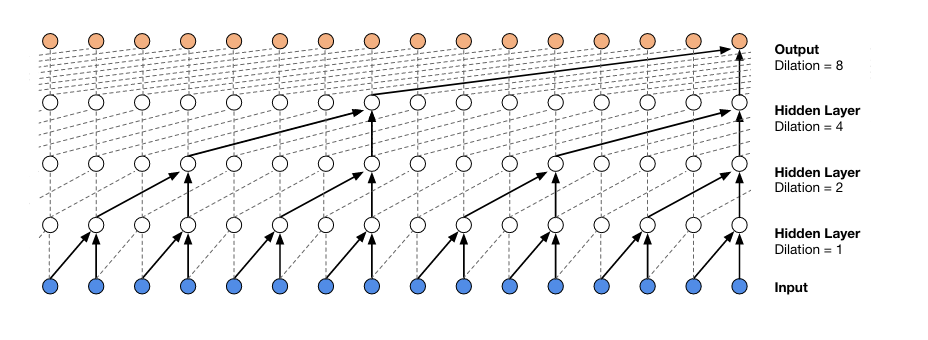
\includegraphics[width=\textwidth]{figures/2-sota/dilated-convolution.png}
    \caption[WaveNet]{\textbf{WaveNet} --- This illustration was taken from \cite{oord_wavenet_2016}. It shows the idea behind WaveNet, applying dilated convolutions to \ac{AR} models.}
    \label{fig:dilated-convolution}
\end{figure}

This structure enables WaveNet to capture long-range dependencies in the input sequence, which is crucial for generating high-quality audio. If an \ac{RNN} (see Section \ref{sec:rnn}) sees only one input sample at each time step, WaveNet has direct access to multiple input samples \cite{huzaifah_deep_2021}. For example, in speech generation, WaveNet can use its sizeable receptive field to model the relationship between a word spoken early in a sentence and its pronunciation later in the sentence.

WaveNet uses a softmax activation function at each output node to produce a probability distribution over the possible values at each time step. During training, the network is fed sequences of input data and their corresponding ground truth values. The model's parameters are adjusted so that its outputs match the ground truth as closely as possible.

WaveNet can use its trained parameters to generate new sequences by sampling from its output probability distribution during generation. This allows it to generate diverse and high-quality outputs, such as realistic human speech or written text, by combining its learned representations of the underlying data distribution with a small amount of randomness.

The input of WaveNet is usually a Mel-Spectrogram (or other representations), and the output is the sound signal.

WaveNet can be conditioned on, for instance, text for \ac{TTS} settings by feeding extra information about the text itself (\textit{e.g.} embeddings). If a model is not conditioned on text, it generates random sounds without any global structure behind it.

The results were astonishing. ``A single WaveNet can capture the characteristics of many different speakers with equal fidelity, and can switch between them by conditioning on the speaker identity. When trained to model music, we find that it generates novel and often highly realistic musical fragments.'' \cite{oord_wavenet_2016}.

Even though this model is good at learning the characteristics of sounds over brief periods, it struggles with global latent structure. They are also very slow for training and inferring \cite{tahiroglu_-terity_2020}.

%%%%%%%%%%%%%%%%%%%%%%%%%%%%%%%%%

\subsubsection{WaveNet Variants} \label{sec:wavenet-variants}

The WaveNet model has emerged as a powerful tool for generating high-quality audio waveforms, particularly for speech and music applications. However, its architecture, which employs dilated convolutions and deep residual networks, can be computationally intensive and challenging to train. To address these limitations, several WaveNet variants have been proposed in recent years that aim to reduce the complexity of the model while maintaining its effectiveness.

One such variant is \textbf{WaveRNN} \cite{kalchbrenner_efficient_2018}, which employs a single \ac{RNN} (see Section \ref{sec:rnn}) to approximate the dilated convolutions in WaveNet. This approach significantly speeds up training time while maintaining the quality of the generated audio. Another variant, FloWaveNet \cite{kim_flowavenet_2018}, employs a flow-based generative model (Section \ref{sec:flow-model}) that allows for efficient training with only one training stage while producing high-quality audio. Additionally, Fast WaveNet  \cite{paine_fast_2016} employs a caching mechanism to reduce the computational cost of the model while maintaining an \ac{AR} structure.

These WaveNet variants are unique in their architectures and training procedures but share the goal of making audio generation more efficient and accessible. While these models are primarily focused on speech and music generation, they can be adapted to other types of audio data. Ongoing research in this area may explore further optimization of these models, integration with other models, and application to new domains.

\subsubsection{MelGAN} \label{sec:melgan}

According to Kumar et al. in 2019, in their \textit{MelGAN} paper~\cite{kumar_melgan_2019}, audio generation with \acp{GAN} is possible although a challenging task (see Section \ref{sec:gan}). Previous studies in this field have encountered difficulties generating coherent raw audio waveforms using \acp{GAN}. Nonetheless, Kumar et al. demonstrate in their \textit{MelGAN} paper that introducing certain architectural changes makes it feasible to train \acp{GAN} to generate high-quality and coherent audio waveforms reliably.

The generator of MelGAN is a fully convolutional feed-forward network that takes a Mel-Spectrogram as input and generates a raw waveform as output. This approach allows for efficient and parallelized processing of audio data.

The decoder takes the waveform and decides whether it is a realistic sound. The decoder is not a single neural network but a multi-scale architecture with three discriminators (D1, D2, D3). These discriminators have identical network structures but operate on different audio scales. D1 operates on the scale of raw audio, while D2 and D3 operate on raw audio downsampled by a factor of 2 and 4, respectively. The use of multiple discriminators at different scales is motivated by the fact that audio has structure at different levels.

MelGAN proved itself way faster than other architectures such as WaveNet (see Section \ref{sec:wavenet}) with comparable results (for inference, roughly thirty-six thousand times faster than WaveNet), given its reduced number of parameters.


%%%%%%%%%%%%%%%%%%%%%%%%%%%%%%%%%

\subsubsection{GANSynth} \label{sec:gansynth}

\textit{GanSynth}, presented in 2019, \cite{engel_gansynth_2019} is a \ac{GAN} (see Section \ref{sec:gan}) that uses log-magnitude spectrograms and phases to generate coherent waveforms. Compared to directly generating waveforms with stridden convolutions, the use of spectrograms and phases has been shown to produce better results.

The study focuses on the NSynth \cite{engel_neural_2017} dataset, a collection of 300 000 musical notes from 1 000 different instruments.

The model first samples a random vector $z$ from a spherical Gaussian distribution. This vector is passed through a stack of transposed convolutions, which upsample and generate output data $x = G(z)$. This generated data is then fed into a discriminator network, which uses downsampling convolutions to estimate a divergence measure between the real and generated distributions.

The architecture of the discriminator network mirrors that of the generator, which allows for a more efficient training process. Optimizing the divergence measure allows the generator to produce spectrograms and phases that resemble actual musical notes more closely.

The study results demonstrate that \acp{GAN} outperform WaveNet (see Section \ref{sec:wavenet}) baselines on automated and human evaluation metrics and can efficiently generate several audio orders of magnitude faster than their \ac{AR} counterparts.

%%%%%%%%%%%%%%%%%%%%%%%%%%%%%%%%%

\subsubsection{HiFi-GAN}

Proposed in 2020, \textit{HiFi-GAN} \cite{kong_hifi-gan_2020} is a \ac{GAN} (see Section \ref{sec:gan}) model that combines efficiency and high-fidelity speech synthesis. HiFi-GAN achieves this by leveraging the periodic patterns inherent in speech audio, demonstrating that modeling these patterns is crucial for enhancing sample quality. The model includes a generator and two discriminators, trained adversarially, and two additional losses for improving training stability and model performance.

The generator is a fully \ac{CNN} (see Section~\ref{sec:CNN}) that takes Mel-Spectrograms as input and upsamples them through transposed convolutions, matching the temporal resolution of raw waveforms. The discriminators are the \ac{MSD} and a \ac{MPD}. \Ac{MSD} evaluates the audio sequence on different scales using a mixture of three convolutional sub-discriminators with different average pools. At the same time, \ac{MPD} consists of small sub-discriminators that capture different implicit structures of input audio by looking at different parts, accepting only equally spaced samples of input audio with different periods. 

HiFi-GAN's performance is evaluated using a subjective human evaluation (\ac{MOS}) on a single speaker dataset, which shows that the proposed method exhibits similarity to human quality. The model achieves a higher \ac{MOS} score than WaveNet (see Section \ref{sec:wavenet}).

Importantly, HiFi-GAN achieves this high-quality synthesis efficiently. Specifically, the model generates 22.05 kHz high-fidelity audio 167.9 times faster than real-time on a single V100 \ac{GPU}, demonstrating superior computational efficiency compared to AR and flow-based models. Moreover, a small-footprint version of HiFi-GAN generates samples 13.4 times faster than real-time on \ac{CPU} with comparable quality to an \ac{AR} counterpart.

\subsection{End-to-End Models} \label{sec:end-to-end}

Audio synthesis is the task of producing artificial audio from text or other kinds of data. Traditionally, audio synthesis systems consist of multiple stages, such as a data analysis frontend, a sound model, and an audio synthesis module. Building these components requires extensive domain expertise and may contain brittle design choices. Moreover, these components are usually trained separately on different objectives and datasets, which may introduce errors and inconsistencies in the final output. To overcome these limitations, end-to-end models have been proposed that directly learn the mapping between text (or other kinds of data) and audio waveform using deep neural networks. These models are presented in this Section.

Existing research establishes two main frameworks for end-to-end models: specialized models designed for a specific domain, and universal models aimed at broader applications. The table \ref{tab:end-to-end-audio-models} shows some examples of these models based on their type, input, output, model architecture, and type of conditioning. Specialized models target either speech or music synthesis, such as Char2wav and Jukebox. Researchers have developed different subsets of technologies within speech and music synthesis models, such as neural codec speech models and discrete diffusion models. Universal models, such as SampleRNN and AudioGen, can generate audio from various inputs and domains, such as text or raw audio seeds.

\begin{table}[ht]
\centering
\caption{A comparison of different end-to-end generative models for audio.}
\begin{tabularx}{\textwidth}{|l|l|X|X|X|}
\hline
\textbf{Model} & \textbf{Type} & \textbf{Input}            & \textbf{Output}                        & \textbf{Model Architecture}                                                      \\ \hline
Char2wav~\cite{sotelo_char2wav_2017}       & Speech        & Text prompt               & Raw audio waveform                     & Encoder-decoder with attention and neural vocoder                                \\ \hline
VALL-E~\cite{wang_neural_2023}         & Speech        & Text and acoustic prompt  & Raw audio waveform                     & Neural codec language model and neural vocoder                                   \\ \hline
Jukebox~\cite{dhariwal_jukebox_2020}        & Music         & Genre, artist, and lyrics & Raw audio waveform                     & Hierarchical VQ-VAE and autoregressive Transformer                               \\ \hline
Riffusion~\cite{forsgren_riffusion_2022}      & Music         & Text prompt               & Raw audio waveform                     & Neural codec language model based on discrete diffusion model and neural vocoder \\ \hline
MusicLM~\cite{agostinelli_musiclm_2023}        & Music         & Text prompt               & Raw audio waveform                     & Neural codec language model and neural vocoder                                   \\ \hline
SampleRNN~\cite{mehri_samplernn_2017}      & General       & None                      & Raw audio waveform                     & Hierarchical RNN and neural vocoder                                              \\ \hline
AudioLM~\cite{borsos_audiolm_2022}        & General       & Text prompt               & Raw audio waveform                     & Hybrid tokenization scheme with Transformer models and neural vocoder            \\ \hline
DiffSound~\cite{yang_diffsound_2022}      & General       & Text prompt               & Mel-spectrogram and raw audio waveform & VQ-VAE, discrete diffusion model, and neural vocoder                             \\ \hline
AudioGen~\cite{kreuk_audiogen_2023}       & General       & Text prompt               & Mel-spectrogram and raw audio waveform & Transformer-based generative model and neural vocoder                            \\ \hline
\end{tabularx}
\label{tab:end-to-end-audio-models}
\end{table}

%%%%%%%%%%%%%%%%%%%%%%%%%%%%%%%%%

\subsubsection{Text-to-Speech} \label{sec:tts}

\Acf{TTS} models are designed to convert written text into synthesized speech. These models use deep neural networks to directly learn the mapping between written text and audio waveform. Leveraging developments in \ac{NLP} and speech synthesis techniques, \ac{TTS} models have made significant progress in generating high-quality, human-like speech from text input. This Section examines some of the notable \ac{TTS} models that have been developed recently.

\paragraph{Char2Wav}

The Char2Wav model, proposed in 2017 \cite{rao_grapheme--phoneme_2015}, serves as a speech synthesis model comprising two distinct components: a reader and a neural vocoder. The reader takes text as inputs and produces a sequence of acoustic features as outputs. The neural vocoder then takes these acoustic features and generates raw waveform samples.

The reader is an attention-based recurrent sequence generator. It is a type of neural network that can generate a sequence of outputs based on a sequence of inputs. In this case, the inputs are text, and the outputs are acoustic features. The generator uses a bidirectional \ac{RNN} (see Section \ref{sec:rnn-variants}) as an encoder and a \ac{RNN} with attention as a decoder. The attention mechanism allows the model to focus on different parts of the input sequence as it generates the output.

Instead of using a traditional vocoder to generate the raw waveform samples, Char2Wav uses a learned parametric neural module. Specifically, it uses a conditional version of SampleRNN (see Section \ref{sec:samplernn} to learn the mapping from vocoder features to audio samples. This allows \textit{Char2Wav} to generate speech directly from the acoustic features without relying on a specific vocoder.

Although no formal proofs or analytical results are presented in this work, the proposed architecture is a significant breakthrough in speech synthesis. By demonstrating the effectiveness of using attention-based recurrent sequence generators and learned parametric neural modules, Char2Wav establishes a solid foundation for future research in this area.
\paragraph{VALL-E}

VALL-E is a language model developed by researchers at Microsoft for \ac{TTS} that treats \ac{TTS} as a conditional language modeling task~\cite{wang_neural_2023}. It generates text based on a given context, where the context in VALL-E is the acoustic tokens and phoneme prompts. VALL-E conditions on these inputs to produce the acoustic token sequence for speech synthesis.

VALL-E comprises two components: an audio codec that generates discrete acoustic tokens from speech waveforms and a neural language model that conditions these tokens and phoneme prompts to generate speech for unseen speakers in a zero-shot setting. The high-level architecture can be seen in Figure~\ref{fig:vall-e}.

\begin{figure}[ht]
    \centering
    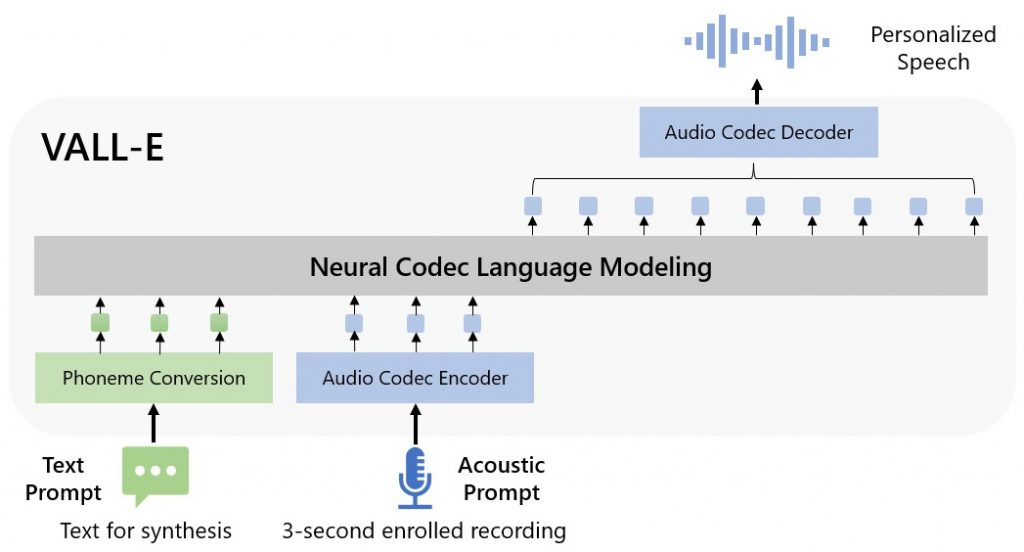
\includegraphics[width=\textwidth]{figures/2-sota/vall-e.jpg}
    \caption[VALL-E]{\textbf{VALL-E} --- The image was extracted from the source publication. It illustrates that both encodings derived from a linguistic prompt and an auditory prompt - provided via the codec encoder - are fed into a language model such as a transformer, and the resulting outputs are passed to the codec decoder to generate audio.}
    \label{fig:vall-e}
\end{figure}

The researchers trained VALL-E using the LibriLight dataset~\cite{kahn_libri-light_2020}, which consists of 60,000 hours of English speech from over 7,000 unique speakers. The proposed approach is robust to noise and generalizes well by leveraging a large and diverse dataset. Previous \ac{TTS} systems are typically trained with fewer data than VALL-E.

VALL-E's performance was evaluated on the LibriSpeech~\cite{panayotov_librispeech_2015} dataset, where all test speakers are unseen during training. VALL-E delivers high performance for speaker-adaptive \ac{TTS} in terms of speech naturalness and speaker similarity, as measured by comparative mean opinion score and similarity mean opinion score, respectively.

Qualitative analysis of VALL-E reveals several interesting findings. Firstly, VALL-E generates speech with diversity. As a result, the same input text can produce different speech outputs. This feature is important for downstream applications such as speech recognition, where diverse inputs with different speakers and acoustic environments are beneficial. The diversity of VALL-E makes it an ideal candidate for generating pseudo-data for speech recognition.

Another finding is that VALL-E maintains the acoustic environment of the prompt during speech synthesis. When the acoustic prompt has reverberation, VALL-E can synthesize speech with reverberation, whereas the baseline outputs clean speech. This can be attributed to VALL-E being trained on a large-scale dataset with diverse acoustic conditions, which allows it to learn acoustic consistency instead of only a clean environment during training.

Furthermore, VALL-E can preserve the emotion in the prompt during speech synthesis. The researchers selected acoustic prompts from the EmoV-DB dataset~\cite{adigwe_emotional_2018}, which contains speech with five emotions. VALL-E kept the exact emotion of the prompt in speech synthesis, even without fine-tuning on an emotional \ac{TTS} dataset.

VALL-E represents a significant advancement in \ac{TTS} technology, with its language model approach and use of audio codec codes as intermediate representations.

In summary, VALL-E is a language model-based \ac{TTS} system that utilizes audio codec codes as intermediate representations. It performs highly in speaker-adaptive \ac{TTS} and demonstrates exciting features such as speech diversity, acoustic environment consistency, and emotion preservation.

\subsubsection{Generative Music}

Generative music is created using generative techniques. End-to-end generative music models enable the production of new musical compositions without using predefined templates or samples, directly from textual or other data inputs. These models use \ac{DL} architectures to capture patterns and structures within different genres or styles of music, and can produce original pieces based on given prompts. This Section explores remarkable generative music models that demonstrate their ability to compose novel musical arrangements.

\paragraph{Jukebox}

Jukebox, a generative model for music that produces music with singing in the raw audio domain, was introduced by Dhariwal et al. in 2020 \cite{dhariwal_jukebox_2020}. The model tackles the long context of raw audio using a multiscale \ac{VQ-VAE} (see Section \ref{sec:ms-vq-vae}) to compress it to discrete codes and models those using \ac{AR} Transformers (see Section \ref{sec:transformers}).

The hierarchical \ac{VQ-VAE} architecture compresses audio into a discrete space, retaining the maximum amount of musical information at increasing compression levels. The model uses residual networks consisting of WaveNet-style (see Section \ref{sec:wavenet}) noncausal 1-D dilated convolutions, interleaved with downsampling and upsampling 1-D convolutions to match different hop lengths. Separate autoencoders with varying hop lengths are trained to maximize the amount of information stored at each level.

After training the \ac{VQ-VAE}, a prior $p(z)$ over the compressed space is learned to generate samples. The prior model is broken up as $p(z) = p(z_{top})p(z_{middle}|z_{top})p(z_{bottom}|z_{middle}, z_{top})$, and separate models are trained for the top-level prior $p(z_{top})$, and upsamplers $p(z_{middle}|z_{top})$ and $p(z_{bottom}|z_{middle}, z_{top})$. Autoregressive Transformers with sparse attention are used for modeling in the discrete token space produced by the \ac{VQ-VAE}.

Jukebox can generate high-fidelity and diverse songs with coherence for up to multiple minutes. It can be conditioned on the artist and genre to steer the musical and vocal style and on unaligned lyrics to make the singing more controllable. The model's release includes thousands of non-cherry-picked samples, model weights, and code.
\paragraph{Riffusion} \label{sec:riffusion}

Riffusion~\cite{forsgren_riffusion_2022} is an open-source model presented in 2022 that generates music clips from text prompts. The model is based on Stable Diffusion (see Section \ref{sec:stable-diffusion}). Riffusion fine-tunes Stable Diffusion to generate images of spectrograms, which can then be converted to music clips.

The authors use \ac{STFT} (see Section \ref{sec:stft}) to compute the spectrogram from audio. The \ac{STFT} is invertible so that the original audio can be reconstructed from a spectrogram. The authors use the Griffin-Lim algorithm~\cite{griffin_signal_1984} to approximate the phase when reconstructing the audio clip.

The authors use diffusion models (see Section \ref{sec:diffusion}) to condition the model's creations on a text prompt and other images, which is helpful for modifying sounds while preserving the structure of an original clip. The authors also use the denoising strength parameter to control how much to deviate from the original clip and towards a new prompt.

So, for inference, the model takes a text prompt as input. Then, the text is encoded into a latent representation using a text encoder. The model generates an image of a spectrogram from the latent representation using a modified version of Stable Diffusion; this is, the Stable Diffusion model fine-tuned for spectrograms. Finally, the generated spectrogram image is converted into an audio clip using the Griffin-Lim algorithm.
\paragraph{MusicLM} \label{sec:musiclm}

MusicLM is a generative model capable of synthesizing high-fidelity music characterized by realistic instrument timbres, accurate pitch, temporal patterns, and smooth transitions between notes based solely on textual descriptions of desired musical attributes (see Section~\ref{sec:musiclm}). The model extends the AudioLM framework for audio generation (see Section~\ref{sec:audiolm}) by incorporating text conditioning via the joint music-text model MuLan (see Section~\ref{sec:mulan}).

MusicLM employs a hierarchical modeling approach with two main stages: semantic modeling and acoustic modeling. The semantic modeling stage uses a Transformer decoder (see Section~\ref{sec:transformers}) to predict semantic tokens from the MuLan audio tokens. Using a separate Transformer decoder, the acoustic modeling stage then predicts acoustic tokens conditioned on both the MuLan audio tokens and predicted semantic tokens. This stage is subdivided into coarse and fine modeling substages to reduce the length of the token sequences, following the AudioLM approach.   

Overall, MusicLM leverages pre-trained audio encoders (SoundStream, w2v-BERT, and  MuLan) to obtain discrete acoustic and semantic tokens as input, after which hierarchical Transformer decoders first predict semantic tokens and then acoustic tokens when conditioned on MuLan text embeddings during synthesis. The hierarchical approach and use of semantic tokens aims to enable coherent long-term generation over extended durations.

MusicLM can generate coherent musical sequences up to 5 minutes in duration, constituting a notable achievement in the context of generative music models. The model captures various musical characteristics specified in textual prompts, including instrument timbre, melodic elements, and musical genre.

The model's performance was assessed using the MusicCaps dataset which comprises 5,500 pairs of music-texts that have been annotated by experts. The dataset includes diverse genres, instruments, and moods. The authors assert that this dataset thoroughly assesses the model's capability to generate various aspects of music from textual prompts. The evaluation metrics comprise human judgments of similarity between the generated outcomes and the prompts, as well as overall quality and others.    

The paper discusses potential limitations, including a proclivity for mode collapse and difficulty generating fine-grained structures over long sequences. However, further investigation is needed to probe the model's limitations and failure modes in greater depth.

In summary, MusicLM represents a promising generative model capable of synthesizing high-fidelity music from textual descriptions via shared embedding spaces and learned associations between text and music encodings, enabling it to capture diverse musical characteristics specified in textual prompts. The MusicCaps dataset provides a valuable means of evaluating the model's performance across various musical styles and prompts.

\subsubsection{General Text-to-Audio}

Text-to-audio systems have a wide range of applications beyond speech synthesis or generative music tasks. End-to-end models convert different forms of textual input into corresponding audio outputs. The outputs have diverse purposes, including sound effects generation, voice transformation, and environmental sound synthesis. These models provide flexible solutions for transforming text into realistic auditory experiences by training on large-scale datasets containing paired text-audio examples across various domains. This Section presents several text-to-audio approaches that demonstrate innovative methods of audio synthesis based on specific textual cues.

\paragraph{SampleRNN} \label{sec:samplernn}

\textit{SampleRNN} is a neural audio generation model proposed in 2017 that can produce high-quality audio samples from scratch \cite{mehri_samplernn_2017}. It uses a hierarchical structure of \acp{RNN} (see Section \ref{sec:rnn}) to model the probability distribution of audio waveforms at different temporal resolutions. The lowest \ac{RNN} operates on individual samples, while higher \acp{RNN} capture longer-term dependencies and structure. SampleRNN can learn from any audio data without any prior knowledge or labels.

The higher \acp{RNN} capture the longer-term dependencies by receiving inputs from lower \acp{RNN} at a lower sampling rate. This way, they can process longer audio sequences. The higher \acp{RNN} also use skip connections to directly access the outputs of lower \acp{RNN}, which helps to avoid vanishing gradients and preserve information across different levels of abstraction.

Each cell is a \ac{RNN} variant, such as \ac{GRU} (see Section \ref{sec:rnn-variants}) that takes as input a frame of audio samples from a lower \ac{RNN} and outputs a hidden state vector that encodes the long-term context of the audio. This output is passed upwards in the hierarchy to other \acp{RNN} that take it. Multiple layers are possible, each operating at a different temporal resolution. All the outputs are then inputted in the final level \ac{RNN}, whose output is the next audio sample based on the combined information from all hierarchy levels.
\paragraph{AudioLM} \label{sec:audiolm}

The framework called AudioLM was introduced by Borsos et al. in 2022 as a means for high-quality audio generation with long-term consistency~\cite{borsos_audiolm_2022}. In this representation space, the framework maps input audio to a sequence of discrete tokens and treats audio generation as a language modeling task. AudioLM achieves high-quality synthesis and long-term structure through a hybrid tokenization scheme. This scheme combines the discretized activations of a masked language model pre-trained on audio (semantic tokens) and the discrete codes produced by a neural audio codec (acoustic tokens).

The AudioLM framework consists of three main components:

\begin{enumerate}
	\item A \textit{tokenizer model} that maps the input audio $x$ into a sequence $y = \text{enc}(x)$ of discrete tokens from a finite vocabulary, with $T' < T$.
	\item A \textit{decoder-only Transformer language model} that operates on the discrete tokens $y$, trained to maximize the likelihood $\prod_{t=1}^{T'} p(y_t|y_{<t})$. The model predicts the token sequence $\hat{y}$ autoregressively at inference time.
	\item A \textit{detokenizer model} that maps the sequence of predicted tokens back to audio, producing the waveform $\hat{x} = \text{dec}(\hat{y})$.
\end{enumerate}

The tokenizer and detokenizer models are pre-trained and frozen before training the language model, simplifying the training setup. The number of tokens $T'$ is significantly smaller than $T$, allowing for increased temporal context size in the language model.

To reconcile the conflicting requirements of high-quality audio reconstruction and capturing long-term dependencies, AudioLM relies on a combination of acoustic and semantic tokens. Acoustic tokens are computed using SoundStream (see Section~\ref{sec:soundstream}). Semantic tokens are computed using w2v-BERT~\cite{chung_w2v-bert_2021}, a model for learning self-supervised audio representations. The semantic tokens enable long-term structural coherence while modeling the acoustic tokens conditioned on the semantic tokens enables high-quality audio synthesis.

AudioLM adopts a hierarchical approach by first modeling the semantic tokens for the entire sequence and then using these as conditioning to predict the acoustic tokens. AudioLM generates syntactically and semantically plausible speech continuations while maintaining speaker identity and prosody for unseen speakers when trained on speech without any transcript or annotation. The approach also extends beyond speech, generating coherent piano music continuations despite being trained without any symbolic representation of music.
\paragraph{DiffSound}

\textit{DiffSound} was presented in a paper, in 2022, that displays a novel text-to-sound generation framework that uses a text encoder, a \ac{VQ-VAE}, a decoder, and a vocoder. The framework takes text as input and outputs synthesized audio corresponding to the input text. The decoder, in particular, is a critical component of the framework, and the paper focuses on designing a suitable decoder, calling it \textit{DiffSound} \cite{yang_diffsound_2022}.

DiffSound is a diffusion decoder (Section \ref{sec:diffusion}) based on the discrete diffusion model. DiffSound predicts all Mel-Spectrogram tokens in one step and then refines the predicted tokens in the next step, resulting in better-predicted results after several steps. It not only produces better text-to-sound generation results compared to an \ac{AR} decoder, but it is also faster, with a generation speed five times faster than an \ac{AR} decoder.

The entire framework acts as this: First, the text is encoded into embeddings using a model like a transformer (Section \ref{sec:transformers}). Then, this representation conditions the generation of spectrogram embeddings using diffusion (the DiffSound model). These embeddings are then passed through the pretrain \ac{VQ-VAE} decoder to generate the spectrogram. The spectrogram runs through a vocoder (Section \ref{sec:vocoders}) to generate the waveform. In the original text, the vocoder used was the MelGAN (see Section \ref{sec:melgan}). This process can be seen in Figure \ref{fig:diffsound}.

\begin{figure}[ht]
    \centering
    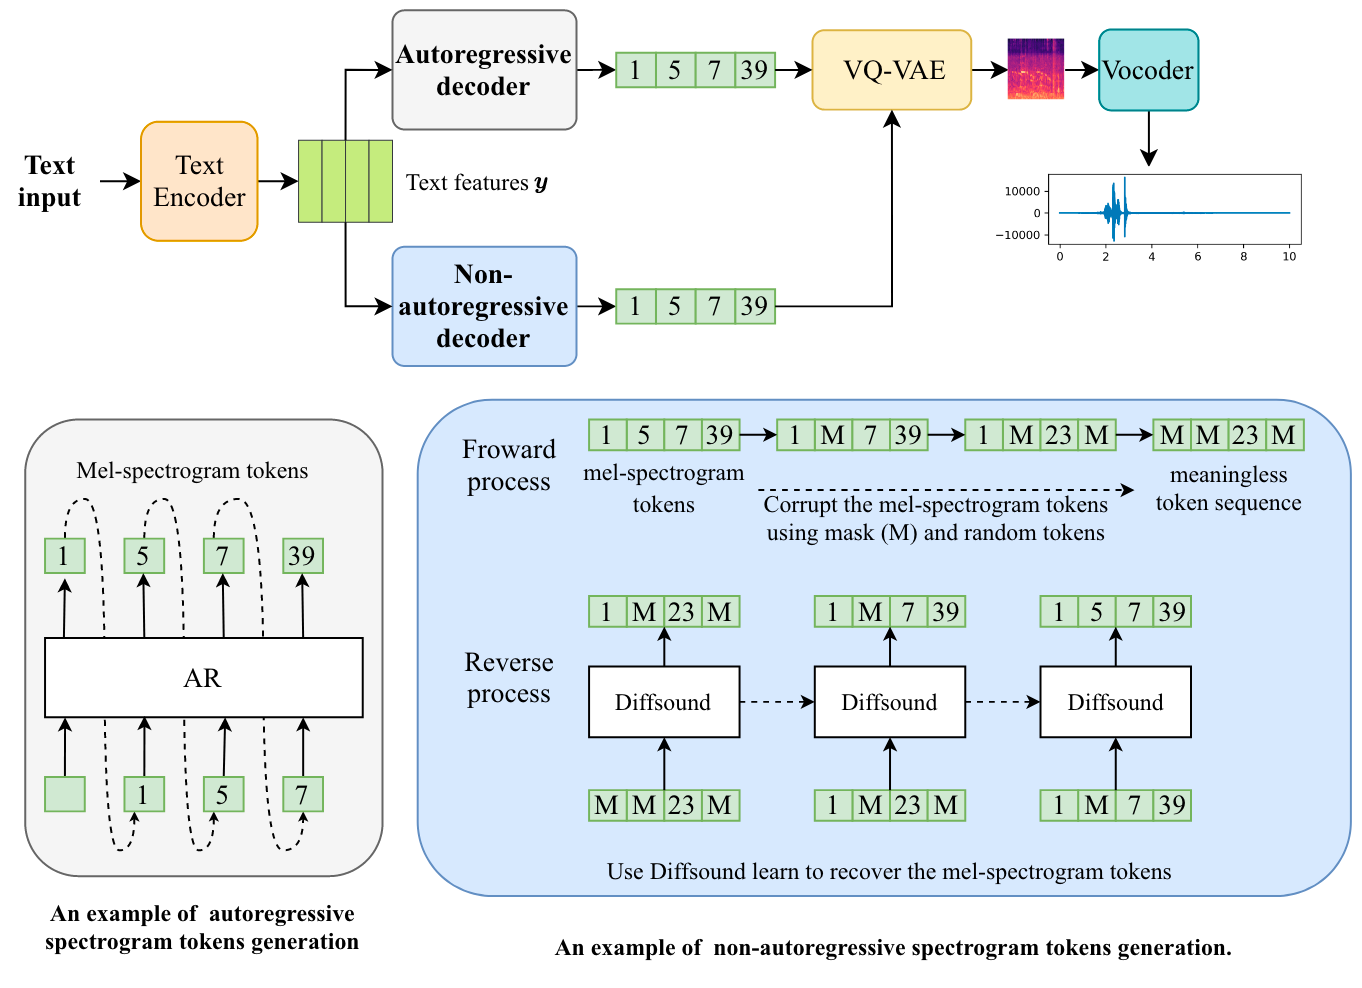
\includegraphics[width=\textwidth]{figures/2-sota/diffsound.png}
    \caption[DiffSound framework]{\textbf{DiffSound framework} --- This illustration was taken from the original paper. At the top, the general framework is present. Two decoders are present, but only one of them is used. The decoder results in a set of latent features. These features are passed to the decoder of the \ac{VQ-VAE} that generates a Mel-Spectrogram (the square with red and blue tones) that, through a vocoder, generates a sound. The two bottom images represent the two decoders. One is a \ac{DARN} (see Section \ref{sec:darn}), the other works with diffusion.}
    \label{fig:diffsound}
\end{figure}
\paragraph{AudioGen} \label{sec:audiogen}

In 2023, Kreuk et al.~\cite{kreuk_audiogen_2023} proposed AudioGen, an auto-regressive generative model that generates audio samples conditioned on text inputs. The model comprises two primary stages: (i) learning a discrete representation of the raw audio using an \ac{AE} method and (ii) training a Transformer language model (see Section~\ref{sec:transformers}) over the learned codes obtained from the audio encoder, conditioned on textual features. During inference, the model samples from the language model generate a new set of audio tokens given text features, which can then be decoded into the waveform domain using the decoder component.

To address the challenge of text-to-audio generation, the authors propose an augmentation technique that mixes different audio samples to train the model to separate multiple sources internally. Furthermore, the authors explore the use of multi-stream modeling for faster inference, allowing the use of shorter sequences while maintaining a similar bitrate and perceptual quality. The proposed method outperforms evaluated baselines over both objective and subjective metrics. Additionally, the authors extend the proposed method to conditional and unconditional audio continuation, demonstrating its ability to generate complex audio compositions.


